\documentclass{article}
\usepackage[utf8]{inputenc}
\usepackage{amsmath}
\usepackage{amssymb}
\usepackage{amsfonts}
\usepackage{amsthm}
\usepackage{parskip}
\usepackage{bm}
\usepackage{tikz}

\usepackage{permute}

\newcommand{\N}{\mathbb{N}}
\newcommand{\Z}{\mathbb{Z}}
\newcommand{\Q}{\mathbb{Q}}
\newcommand{\R}{\mathbb{R}}
\newcommand{\C}{\mathbb{C}}
\newcommand{\gen}[1]{\left\langle #1 \right\rangle}
\DeclareMathOperator*{\sgn}{sgn}
\DeclareMathOperator*{\ord}{ord}

\newenvironment{hwproof}[1]
{
    #1
    \begin{proof}
}{
    \end{proof}
}

% Lauritzen Chapter 2: Exercises 40, 41, 43, question not from book
\title{HW7}
\author{Asier Garcia Ruiz}

\begin{document}
\maketitle

\section*{Chapter 2}
\subsection*{Ex. 40}
\begin{hwproof}
    {
        Let $\sigma \in S_5$ denote the 5-cycle
        \begin{equation*}
            \pmt{(12345)} = \begin{pmatrix}
                1 & 2 & 3 & 4 & 5  \\
                2 & 3 & 4 & 5 & 1.
            \end{pmatrix}
        \end{equation*}

        (i) Show that $\sigma$ is an even permutation and that
        $\gen{\sigma} = \{\sigma^n : n \in \Z\}$ has order 5 and write down the
        elements in $\gen{\sigma}$

    }
    We can see that the set of inversions of $\sigma$ is
    \begin{equation*}
        I_\sigma = \{(1,5),(2,5),(3,5),(4,5))\}.
    \end{equation*}
    Clearly, $|I_\sigma| = 4$ and thus $\sgn(\sigma) = (-1)^4 = 1$. Therefore,
    the permutation is even.

    The elements of $\gen{\sigma}$ are
    \begin{equation*}
        \gen{\sigma} = \{id, (12345), (13524), (14253), (15432)\}.
    \end{equation*}
\end{hwproof}

\begin{hwproof}
    {
        (ii) Prove the $\gen{\sigma}$ is not a normal subgroup of $S_5$.
    }

    We can see that
    \begin{equation*}
        (134)\gen{\sigma}(134)^{-1} =
        \{\pmt{(134)()(143)},\pmt{(134)(12345)(143)}, \pmt{(134)(13524)(143)},
        \pmt{(134)(14253)(143)}, \pmt{(134)(15432)(143)}\} \neq \gen{\sigma}.
    \end{equation*}
    Therefore, this is not a normal group of $S_4$.
\end{hwproof}

\subsection*{Ex. 41}
\begin{hwproof}
    {
        (i) Let $\sigma, \tau \in S_4$. Show that
        $\sgn(\tau\sigma\tau^{-1}) = \sgn(\sigma)$.
    }

    We know that the sign of a permutation is a group homomorphism. Hence we can
    write
    \begin{equation*}
        \sgn(\tau \sigma \tau^{-1}) = \sgn(\tau)\sgn(\sigma)\sgn(\tau^{-1}).
    \end{equation*}
    Furthermore, since the composition on the image of $\sgn$ is multiplication,
    we have that elements are abelian in the image. Combining this with the fact
    that $\sgn(\tau^{-1}) = \sgn(\tau)^{-1}$ we get that
    \begin{equation*}
        \sgn(\tau)\sgn(\sigma)\sgn(\tau^{-1}) = \sgn(\tau)\sgn(\tau)^{-1}\sgn(\sigma)
        = \sgn(\sigma).
    \end{equation*}
    Therefore, we have that
    \begin{equation*}
        \sgn(\tau\sigma\tau^{-1}) = \sgn(\sigma)
    \end{equation*}
    as required.
\end{hwproof}

\begin{hwproof}
    {
        (ii) Write the 3-cycle $\pmt{(123)}$ as a product of two simple transpositions.
        Prove that for a general 3-cycle $\sigma$ one can find a permutation
        $\tau \in S_4$ such that $\tau \sigma \tau^{-1} = \pmt{(123)}$. Use this to show
        that 3-cycles in $S_4$ are even. Prove that a 3-cycle has order 3 in $A_4$.
    }

    The 3-cycle $(123)$ can be written as the product of $(12)(23)$.

    Let $\sigma$ be a general 3 cycle. Since
    $S_4$ is a group we know that composition is closed and every element has an inverse
    in $S_4$. We also know that $S_4$ is generated by simple transpositions, and
    that any permutation is a product of simple transpositions.
    Hence, we are guaranteed that for some $\tau \in S_4$
    \begin{equation*}
        \sigma = \tau^{-1} (123) \tau
    \end{equation*}
    and thus
    \begin{equation*}
        \tau \sigma \tau^{-1} = (123)
    \end{equation*}

    We know from part (ii) that $\sgn(\tau \sigma \tau^{-1}) = \sgn(\sigma)$ and
    thus
    \begin{equation*}
        \sgn(\sigma) = \sgn(\tau(123)\tau^{-1}) = \sgn((123)) = 2.
    \end{equation*}
    Therfore any 3-cycle is even.

    Let $\sigma \in A_4$ be a 3-cycle in $A_4$. We know that for some $\tau \in A_4$
    we have that $\sigma = \tau (123) \tau^{-1}$. Now we can compute
    \begin{align*}
        \sigma^3 & = (\tau (123) \tau^{-1})^3                                            \\
                 & = (\tau (123) \tau^{-1})(\tau (123) \tau^{-1})(\tau (123) \tau^{-1}), \\
                 & = \tau (123)(123)(123)\tau^{-1},                                      \\
                 & = \tau \ id \ \tau^{-1} = id.
    \end{align*}
    Therefore, every 3-cycle has order 3 in $A_4$.
\end{hwproof}

\begin{hwproof}
    {
        (iii) Show that the number of 3-cycles in $A_4$ is greater than six. Conclude
        that the only subgroup of $A_4$ containig every 3-cycle is $A_4$.
    }
\end{hwproof}

We know that $|A_4| = \frac{4!}{2} = 12$. Since the order of any subgroup must
divide the order of the group (Lagrange's Thm.), it is sufficient to show there
are more than five 3-cycles in $A_4$ (since the identity must also be in the subgroup).
In fact, we observe that
\begin{equation*}
    (234), (243), (123), (124),(132),(134) \in A_4.
\end{equation*}
Therefore, since there are more than 5 3-cycles in $A_4$, we have that the only
subgroup of $A_4$ containing every 3-cycle is itself as required.

\begin{hwproof}
    {
        (iv) Let $\varphi: A_4 \to \Z / 2\Z$ be a group homomorphism. Show that if
        $\sigma$ is a 3-cycle then $\varphi(\sigma) = [0] = 2\Z \in \Z / 2\Z$.
        Use this to prove that $\varphi(\sigma) = [0]$ for every
        $\sigma \in A_4$.
    }

    Since $\sigma$ has order 3 in $A_4$ we know that
    \begin{equation*}
        \varphi(\sigma^3) = \varphi(id_{A_4}) = [0].
    \end{equation*}

    Now assume, for the sake of contradiction, that $\varphi(\sigma) \neq [0]$.
    Since there are only two elements in $\Z / 2\Z$, this means that
    $\varphi(\sigma) = [1]$. This implies that
    \begin{equation*}
        \varphi(\sigma^3) = \varphi(\sigma)\varphi(\sigma)\varphi(\sigma)
        = [1] + [1] + [1] = [1].
    \end{equation*}
    This is a contradiction, and thus we have that $\varphi(\sigma) = [0]$
    as required.

    We know from (ii) that $(123) \in A_4$ and that any $\sigma \in A_4$ is
    such that $\sigma = \tau (123) \tau^{-1}$. Furthermore, we know now that
    since $(123)$ is a 3-cycle then $\varphi((123)) = [0]$. This allows us to
    say
    \begin{equation*}
        \varphi(\sigma) = \varphi(\tau (123) \tau^{-1})
        = \varphi(\tau) \varphi((123)) \varphi(\tau^{-1})
        = \varphi(\tau) + [0] + \varphi(\tau)^{-1}
        = [0]
    \end{equation*}
    as required.
\end{hwproof}

\begin{hwproof}
    {
        Prove that $A_4$ does not contain a subgroup of order 6.
    }
    Suppose that $H \leq A_4$ such that $|H| = 6$. Let $\sigma$ be a 3-cycle
    not in $H$. Now consider the cosets $H, \sigma H, \sigma^2 H \in A_4 / H$.
    Since $A_4 / H = [A_4 : H] = 2$, two of these cosets must be equal.
    Clearly $H \neq \sigma H$, so either $\sigma^2 H = H$ or $\sigma^2 H = \sigma H$.

    If $H = \sigma^2 H$, then $\sigma^2 = \sigma^{-1} \in H$. This implies that
    $\sigma \in H$, a contradiction. Similarly if $\sigma^2 H = \sigma H$ then
    $\sigma \in H$, a contradiction. So $H$ does not exist.

\end{hwproof}

\subsection*{Ex. 43}
\begin{hwproof}
    {
        Write
        \begin{equation*}
            \sigma = \begin{pmatrix}
                1 & 2 & 3 & 4 & 5 & 6 \\
                6 & 5 & 4 & 3 & 2 & 1
            \end{pmatrix}
            \in S_6
        \end{equation*}
        as a product of the minimal number of simple transpositions.
    }

    We can write
    \begin{equation*}
        \sigma = (12)(23)(34)(45)(56)(12)(23)(34)(45)(12)(23)(34)(12)(23)(12)
    \end{equation*}
\end{hwproof}




\section*{Out of book}
\begin{hwproof}{
        Draw the Cayley graph for $S_4$ generated by the simple transpositions
        $\pmt{(12)}$, $\pmt{(23)}$, $\pmt{(34)}$.
    }
    Let the red, green, and blue lines represent multiplication by $(12), (23)$ and $(34)$
    respectively. We then have the Cayley graph:

    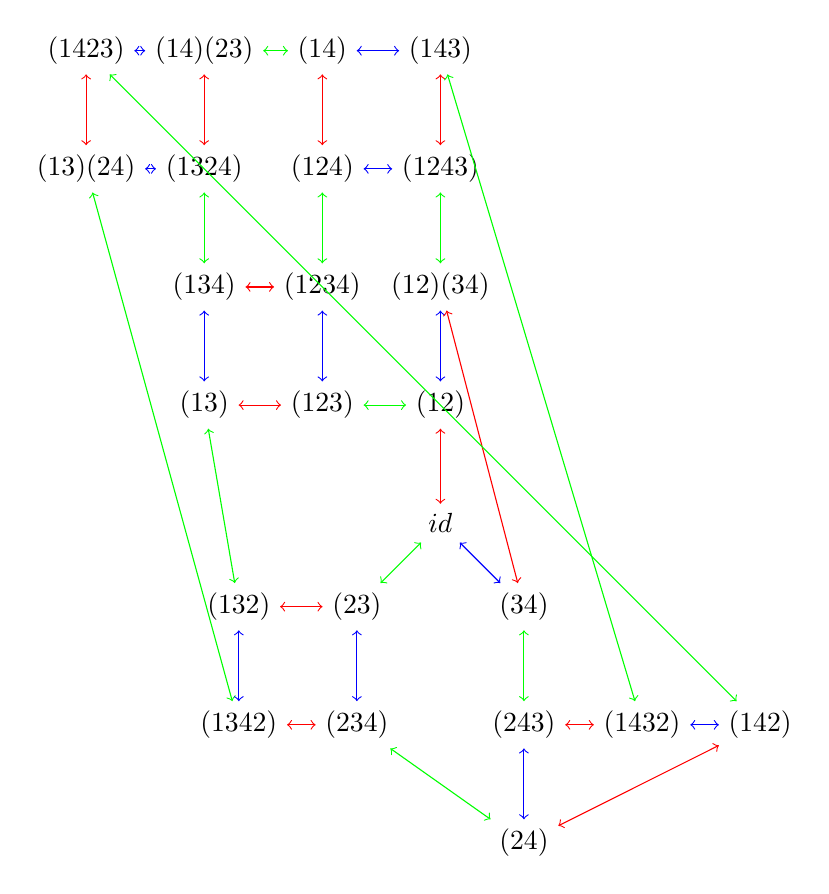
\begin{tikzpicture}[main/.style = {draw, circle}, node distance=1.5cm]

        \node[] (id) {$id$};

        \node[] (12) [above of=id] {$(12)$};
        \node[] (23) [below left of=id] {$(23)$};
        \node[] (34) [below right of=id] {$(34)$};
        \draw [to-to, red] (id) -- (12);
        \draw [to-to, green] (id) -- (23);
        \draw [to-to, blue] (id) -- (34);

        \node[] (234) [below of=23] {$\pmt{(23)(34)}$};
        \node[] (132) [left of=23] {$\pmt{(23)(12)}$};
        \draw [to-to, blue] (23) -- (234);
        \draw [to-to, red] (23) -- (132);

        \node[] (243) [below of=34] {$\pmt{(34)(23)}$};
        \draw [to-to, green] (34) -- (243);

        \node[] (1342) [left of=234] {$\pmt{(234)(12)}$};
        \draw [to-to, red] (234) -- (1342);

        \node[] (24) [below of=243] {$\pmt{(243)(34)}$};
        \node[] (1432) [right of=243] {$\pmt{(243)(12)}$};
        \draw [to-to, blue] (243) -- (24);
        \draw [to-to, red] (243) -- (1432);

        \node[] (142) [right of=1432] {$\pmt{(1432)(34)}$};
        \draw [to-to, blue] (1432) -- (142);

        \node[] (123) [left of=12] {$\pmt{(12)(23)}$};
        \node[] (12n34) [above of=12] {$\pmt{(12)(34)}$};
        \draw [to-to, green] (12) -- (123);
        \draw [to-to, blue] (12) -- (12n34);

        \node[] (13) [left of=123] {$\pmt{(123)(12)}$};
        \node[] (1234) [above of=123] {$\pmt{(123)(34)}$};
        \draw [to-to, red] (123) -- (13);
        \draw [to-to, blue] (123) -- (1234);

        \node[] (134) [left of=1234] {$\pmt{(1234)(12)}$};
        \draw [to-to, red] (1234) -- (134);

        \node[] (1243) [above of=12n34] {$\pmt{(12)(34)(23)}$};
        \draw [to-to, green] (1243) -- (12n34);

        \node[] (143) [above of=1243] {$\pmt{(1243)(12)}$};
        \node[] (124) [left of=1243] {$\pmt{(1243)(34)}$};
        \draw [to-to, blue] (124) -- (1243);
        \draw [to-to, red] (143) -- (1243);

        \node[] (14) [left of=143] {$\pmt{(143)(34)}$};
        \draw [to-to, blue] (143) -- (14);

        \node[] (14n23) [left of=14] {$\pmt{(14)(23)}$};
        \draw [to-to, green] (14) -- (14n23);

        \node[] (1324) [below of=14n23] {$\pmt{(14)(23)(12)}$};
        \node[] (1423) [left of=14n23] {$\pmt{(14)(23)(34)}$};
        \draw [to-to, red] (14n23) -- (1324);
        \draw [to-to, blue] (14n23) -- (1423);

        \node[] (13n24) [left of=1324] {$\pmt{(1324)(34)}$};
        \draw [to-to, blue] (1324) -- (13n24);

        % Not assoc'd with new node
        \draw [to-to, red, bend left] (12n34) -- (34);
        \draw [to-to, green, bend left] (143) -- (1432);
        \draw [to-to, red] (14) -- (124);
        \draw [to-to, green] (124) -- (1234);
        \draw [to-to, green] (134) -- (1324);
        \draw [to-to, blue] (134) -- (13);
        \draw [to-to, green] (13) -- (132);
        \draw [to-to, red] (24) -- (142);
        \draw [to-to, green] (24) -- (234);
        \draw [to-to, green] (142) -- (1423);
        \draw [to-to, green] (1342) -- (13n24);
        \draw [to-to, blue] (1342) -- (132);
        \draw [to-to, red] (13n24) -- (1423);
    \end{tikzpicture}
\end{hwproof}

\end{document}
